%%
%% 2019 07 04 Ph. G. Freimann
%%
\newpage
\section{Allgemeines Dreieck}\index{Dreieck!allgemeines}
\sectuntertitel{Alle Ecken stumpf und spitz}

%%%%%%%%%%%%%%%%%%%%%%%%%%%%%%%%%%%%%%%%%%%%%%%%%%%%%%%%%%%%%%%%%%%%%%%%%%%%%%%%%
\subsection*{Lernziele}

\begin{itemize}
 \item Sinussatz\TALS{\cite{frommenwiler18geom} S. 104 Kap. 2.2.2}
 \item Cosinussatz\TALS{\cite{frommenwiler18geom} S. 106 Kap. 2.2.3}
\end{itemize}

\subsection{Sinussatz}\index{Sinussatz}

\begin{gesetz}{Sinussatz}{}
$$\frac{a}{\sin(\alpha)} = \frac{b}{\sin(\beta)} = \frac{c}{\sin(\gamma)}$$
\end{gesetz}

Herleitung:\\

%% Erestzen durch bbwCenterGraphics?
\bbwCenterGraphic{5cm}{tals/trig2/img/Sinussatz.png}
%\raisebox{-1cm}{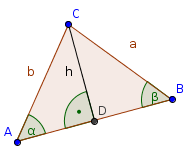
\includegraphics[width=5cm]{img/Sinussatz.png}}

\TNT{3.2}{Zeichne die Höhe ein und betrachte beide rechtwinkligen
  Dreiecke:
  Es gilt nach Definition (Gegenkathete durch Hypothenuse):\\
  $\frac{h}{b}=\sin(\alpha)$ und $\frac{h}{a}=\sin(\beta)$
  somit\\
  $b\sin(\alpha)=h=a\sin(\beta)$
  somit:\\
  $\frac{a}{\sin(\alpha)} = \frac{b}{\sin(\beta)}$
}%% END TNT
\newpage

\subsection*{Aufgaben}
\TALSGeomAadB{104}{95. 97. 98. a) d) f) 102.}

\newpage
\TALS{Den \textbf{Sinussatz} können Sie auch im Taschenrechner
  abspeichern und jederzeit verwenden, indem Sie nur die gegebenen
  Größen verändern (hier: Aufgabe 98. b) Seite 104):

\begin{center}
  \raisebox{-1cm}{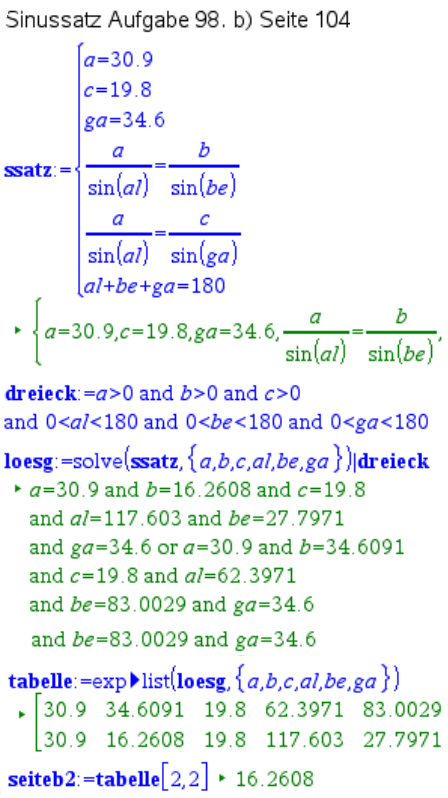
\includegraphics[width=10cm]{tals/trig2/img/sinussatz_ti_nspire.png}}
  \end{center}%%
}%%

\newpage
\subsection{Cosinussatz}\index{Kosinussatz}\index{Cosinussatz}

(auch Kosinussatz)

\begin{gesetz}{Cosinussatz}{}
$$c^2 = a^2 + b^2 - 2ab\cos{(\gamma)}$$
\end{gesetz}

Herleitung:\\

\bbwCenterGraphic{8cm}{tals/trig2/img/Kosinussatz.png}
%\raisebox{-1cm}{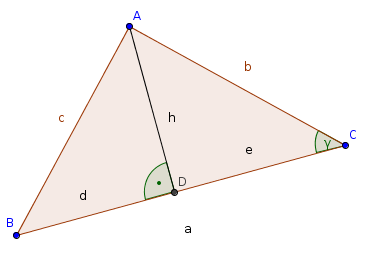
\includegraphics[width=8cm]{img/Kosinussatz.png}}

\noTRAINER{\noteLines{8}}
\TRAINER{Zeichne die Höhe ein und betrachte beide rechtwinkligen
  Dreiecke:
  $e+d=a$\\
  $d=a-e$\\
  $d^2=(a-e)^2=a^2-2ae+e^2$\\
  zudem (Pythagoras):\\
  $e^2 + h^2 = b^2$ und $d^2+h^2 = c^2$\\
  Zweite Gleichung minus erste:\\
  $c^2 - b^2 = d^2 + h^2 - (e^2 + h^2) = d^2 - e^2$
  $d^2$ einsetzen:
  $c^2 - b^2 = (a^2-2ae+e^2) -e^2 = a^2-2ae$\\
  Es gilt (Def. Kosinus) $e=b\cos(\gamma)$ und somit:\\
  $c^2 = b^2 + a^2 -2ab\cos(\gamma)$
}

Gilt dies auch im rechtwinkligen Dreieck?
\TRAINER{ja: $\cos(90) = 0$}
\noTRAINER{\vspace{2cm}}
\subsection*{Aufgaben}
\TALSGeomAadB{106 ff.}{108. 109. 111. a) b) d) f)
114. a)}
\TALS{Bemerkung zu 114. a): Im Buch sind falsche Ziffern
angegeben. Korrekt gerundet wäre es: $\gamma\approx64.1^\circ$,
$c\approx16.7cm$, $\alpha\approx60.0^\circ\approx59.98^\circ$, $\beta\approx
55.9^\circ{}$}

%%\GESOAadB{????}{????}
